\documentclass[../master/master.tex]{subfiles}

\begin{document}

%----------------------------------------------------------------------
% MIDTERM REVIEW
%----------------------------------------------------------------------
\renewcommand{\lecturenum}{R}
\renewcommand{\lecturedate}{Spring 2026}
\renewcommand{\lecturetopic}{Midterm Review}

\section{Midterm Review}

\begin{lecturesummary}
\textbf{Midterm Review:} This document covers key exam-style questions spanning Lectures 1--6. For each problem, we recall the relevant definitions and theorems from class, provide visual intuition, and outline a proof strategy---without writing the full proof.
\end{lecturesummary}

\begin{notebox}
\textbf{Tips for the Exam:}
\begin{itemize}
    \item You do \textbf{not} have to prove a given hint unless otherwise specified.
    \item You do \textbf{not} have to do the problems in order.
    \item Shorthand notations are fine (e.g.\ $\forall$, $\exists$, $\Rightarrow$, $\Leftrightarrow$) as long as your meaning is clear.
    \item You may use \textbf{any equivalent definition} as long as it is correct.
    \item \textbf{1 page} printed/typed cheat sheet allowed.
\end{itemize}
\end{notebox}

%======================================================================
% QUESTION 1
%======================================================================
\subsection{Question 1: ``$\Q$ is dense in $\R$'' and ``$\R$ is the completion of $\Q$''}

\begin{summarybox}
\textbf{Question:} Explain the meaning of ``$\Q$ is dense in $\R$'' and ``$\R$ is the completion of $\Q$.''
\end{summarybox}

\subsubsection*{Part 1: ``$\Q$ is dense in $\R$''}

\textbf{Definition (Density of $\Q$ in $\R$, Lecture 2).}
$\Q$ is \defn{dense} in $\R$ means: for every $a, b \in \R$ with $a < b$, there exists $q \in \Q$ such that $a < q < b$.

In other words, \emph{between any two distinct real numbers, no matter how close together, there is always a rational number sitting between them.} There is no ``gap'' in $\R$ that is free of rationals.

\begin{center}
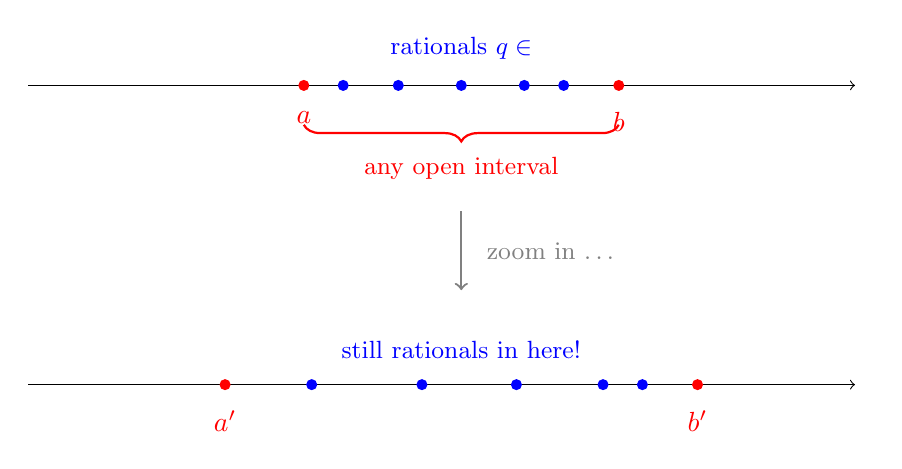
\begin{tikzpicture}[scale=1.0]
    % Number line
    \draw[->] (-0.5,0) -- (10,0) node[right] {$\R$};

    % Points a and b
    \fill[red] (3,0) circle (2pt) node[below=6pt] {$a$};
    \fill[red] (7,0) circle (2pt) node[below=6pt] {$b$};

    % The interval (a,b)
    \draw[thick, red, decorate, decoration={brace, amplitude=6pt, mirror}] (3,-0.5) -- (7,-0.5)
        node[midway, below=8pt] {\small any open interval};

    % Rational points in between
    \fill[blue] (4.2,0) circle (2pt);
    \fill[blue] (5.0,0) circle (2pt);
    \fill[blue] (5.8,0) circle (2pt);
    \fill[blue] (6.3,0) circle (2pt);
    \fill[blue] (3.5,0) circle (2pt);

    % Label
    \node[blue, above=6pt] at (5,0) {\small rationals $q \in \Q$};

    % Zoom
    \draw[->, thick, gray] (5, -1.6) -- (5, -2.6);
    \node[gray, right] at (5.2,-2.1) {\small zoom in \ldots};

    % Zoomed number line
    \begin{scope}[yshift=-3.8cm]
        \draw[->] (-0.5,0) -- (10,0);
        \fill[red] (2,0) circle (2pt) node[below=6pt] {$a'$};
        \fill[red] (8,0) circle (2pt) node[below=6pt] {$b'$};
        \fill[blue] (3.1,0) circle (2pt);
        \fill[blue] (4.5,0) circle (2pt);
        \fill[blue] (5.7,0) circle (2pt);
        \fill[blue] (6.8,0) circle (2pt);
        \fill[blue] (7.3,0) circle (2pt);
        \node[blue, above=6pt] at (5,0) {\small still rationals in here!};
    \end{scope}
\end{tikzpicture}
\end{center}

No matter how far you zoom in on the number line, you will always find rational numbers. You can never isolate an interval of pure irrationals.

\begin{notebox}
\textbf{How density is proved (Lecture 2).} The proof relies on the \textbf{Archimedean property}: for any $x, y \in \R$ with $x > 0$, there exists $n \in \N$ with $nx > y$.

The strategy:
\begin{enumerate}
    \item Since $b - a > 0$, apply the Archimedean property to find $n \in \N$ with $n(b - a) > 1$.
    \item This means $nb - na > 1$, so there is an integer $m$ with $na < m < nb$.
    \item Then $q = \frac{m}{n} \in \Q$ satisfies $a < q < b$.
\end{enumerate}
The key insight: the Archimedean property lets you ``scale up'' any tiny interval $(a,b)$ until it is wide enough (width $> 1$) to guarantee an integer lands inside. Then you scale back down to get a rational.
\end{notebox}

\textbf{Equivalent topological viewpoint.} In Lecture 4, we defined the \defn{closure} of a set $E$ as the smallest closed set containing $E$. Equivalently, $x \in \overline{E}$ if and only if every neighborhood of $x$ intersects $E$. Saying ``$\Q$ is dense in $\R$'' is the same as saying:
\[
\overline{\Q} = \R
\]
That is, every real number is either rational or a limit point of the rationals. For any $x \in \R$ and any $\eps > 0$, the ball $B(x, \eps) = (x - \eps, x + \eps)$ contains a rational number.

\subsubsection*{Part 2: ``$\R$ is the completion of $\Q$''}

This phrase captures a different idea: $\Q$ has ``gaps'' (missing points), and $\R$ is what you get when you fill them all in.

\textbf{The gap in $\Q$ (Lecture 1).} Consider the sets
\[
A = \{p \in \Q : p > 0,\; p^2 < 2\}, \qquad B = \{p \in \Q : p > 0,\; p^2 > 2\}.
\]
We proved that $A$ has no largest element and $B$ has no smallest element. The ``number'' $\sqrt{2}$ that should separate them simply does not exist in $\Q$. So $A$ is bounded above in $\Q$, yet $\sup A$ does not exist in $\Q$.

\begin{center}
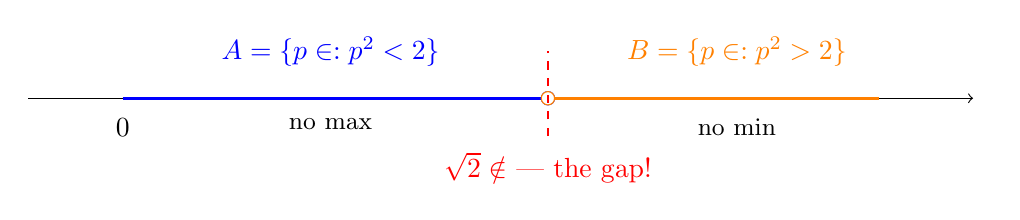
\begin{tikzpicture}[scale=1.2]
    % Number line
    \draw[->] (0,0) -- (10,0) node[right] {$\Q$};

    % Set A
    \draw[very thick, blue] (1,0) -- (5.5,0);
    \draw[blue, fill=white] (5.5,0) circle (2pt);
    \node[blue, above=8pt] at (3.2,0) {$A = \{p \in \Q : p^2 < 2\}$};

    % Set B
    \draw[very thick, orange] (5.5,0) -- (9,0);
    \draw[orange, fill=white] (5.5,0) circle (2pt);
    \node[orange, above=8pt] at (7.5,0) {$B = \{p \in \Q : p^2 > 2\}$};

    % The gap
    \draw[thick, red, dashed] (5.5,-0.4) -- (5.5,0.5);

    % Labels below the line
    \node[below=4pt] at (1,0) {$0$};
    \node[below=4pt] at (3.2,0) {\small no max};
    \node[below=4pt] at (7.5,0) {\small no min};
    \node[red, below=16pt] at (5.5,0) {$\sqrt{2} \notin \Q$ --- the gap!};
\end{tikzpicture}
\end{center}

This is precisely the failure of the \textbf{Least Upper Bound Property} in $\Q$: there exists a nonempty, bounded-above subset of $\Q$ whose supremum does not exist in $\Q$.

\textbf{Definition (LUBP, Lecture 1).} An ordered set $S$ has the \defn{Least Upper Bound Property} if every nonempty subset $E \subseteq S$ that is bounded above has $\sup E \in S$.

\textbf{How $\R$ fills the gaps (Lecture 2).} We construct $\R$ via \defn{Dedekind cuts}: a cut is a nonempty, proper, downward-closed subset $\alpha \subset \Q$ with no maximum. Each cut represents a real number by encoding ``everything to its left.''

\begin{center}
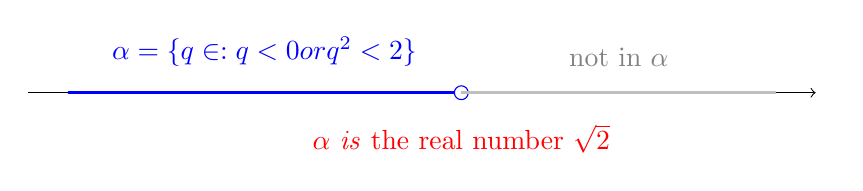
\begin{tikzpicture}[scale=1.0]
    % Number line for Q
    \draw[->] (0,0) -- (10,0) node[right] {$\Q$};

    % The cut for sqrt(2)
    \draw[very thick, blue] (0.5,0) -- (5.5,0);
    \draw[blue, fill=white] (5.5,0) circle (2.5pt);

    % Right side
    \draw[very thick, gray!50] (5.5,0) -- (9.5,0);

    % Labels
    \node[blue, above=6pt] at (3,0) {$\alpha = \{q \in \Q : q < 0 \text{ or } q^2 < 2\}$};
    \node[gray, above=6pt] at (7.5,0) {not in $\alpha$};

    % The ``new point''
    \node[red, below=8pt] at (5.5,0) {$\alpha$ \emph{is} the real number $\sqrt{2}$};
\end{tikzpicture}
\end{center}

The set of all Dedekind cuts forms an ordered field $\R$ that:
\begin{enumerate}
    \item \textbf{Contains $\Q$:} each rational $p$ corresponds to the cut $p^* = \{q \in \Q : q < p\}$.
    \item \textbf{Has the LUBP:} for any nonempty bounded-above collection of cuts, $\sup E = \bigcup_{\alpha \in E} \alpha$ is again a cut (Lecture 2).
    \item \textbf{Is minimal:} $\Q$ is dense in $\R$, so $\R$ adds no ``extra'' points beyond what is needed to fill the gaps.
\end{enumerate}

\begin{notebox}
\textbf{Summary: density vs.\ completion.}
\begin{center}
\renewcommand{\arraystretch}{1.4}
\begin{tabular}{|c|p{5.5cm}|p{5.5cm}|}
\hline
& \textbf{``$\Q$ is dense in $\R$''} & \textbf{``$\R$ is the completion of $\Q$''} \\
\hline
\textbf{Says} & Between any two reals there is a rational. & $\R$ is $\Q$ with all ``gaps'' filled in. \\
\hline
\textbf{Formal} & $\overline{\Q} = \R$ (closure in the metric topology). & $\R$ is an ordered field containing $\Q$ that satisfies the LUBP. \\
\hline
\textbf{Key tool} & Archimedean property. & Dedekind cuts (or Cauchy sequences). \\
\hline
\textbf{Direction} & Starts from $\R$, looks ``down'' at $\Q$ inside it. & Starts from $\Q$, builds ``up'' to $\R$. \\
\hline
\end{tabular}
\end{center}

Density says $\Q$ is \emph{everywhere} in $\R$. Completion says $\R$ is the \emph{smallest} ordered field containing $\Q$ with no gaps (i.e., satisfying the LUBP). Together: $\R$ is built from $\Q$ by filling in the missing suprema, and the original rationals remain spread throughout.
\end{notebox}

\newpage
%======================================================================
% QUESTION 2
%======================================================================
\subsection{Question 2: Open vs.\ Closed Sets; Characterizing Open Sets in Metric Spaces}

\begin{summarybox}
\textbf{Question:} What is the relation between open and closed sets? Characterize open sets in metric spaces.
\end{summarybox}

\subsubsection*{Open and Closed Sets are Complements}

\textbf{Definition (Lecture 4).} Let $X$ be a topological space with topology $\mathcal{T}$.
\begin{itemize}
    \item A set $U \subseteq X$ is \defn{open} if $U \in \mathcal{T}$.
    \item A set $C \subseteq X$ is \defn{closed} if its complement $X \setminus C$ is open.
\end{itemize}

The relationship is definitional: \emph{closed means complement is open.} They are dual notions, not opposites. A set can be both open and closed (e.g., $\emptyset$ and $X$), or neither (e.g., $[0,1)$ in $\R$).

\begin{center}
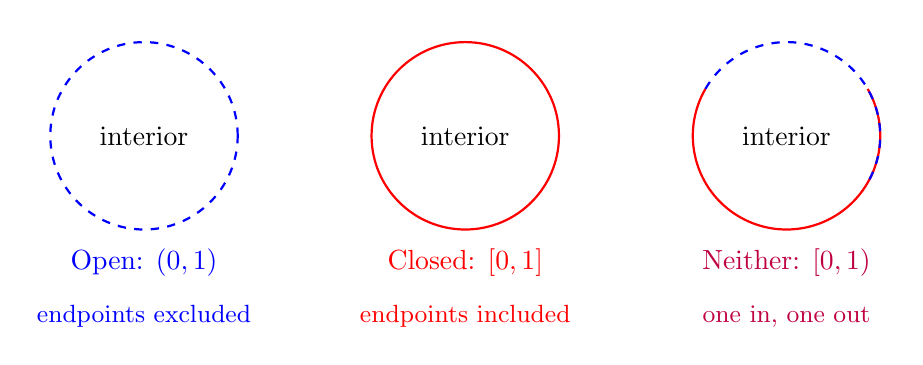
\begin{tikzpicture}[scale=0.85]
    % Open set
    \begin{scope}[xshift=0cm]
        \draw[thick, blue, dashed] (0,0) circle (1.4);
        \node[blue] at (0,-1.9) {Open: $(0,1)$};
        \node at (0,0) {interior};
        \node[blue] at (0,-2.7) {\small endpoints excluded};
    \end{scope}

    % Closed set
    \begin{scope}[xshift=4.8cm]
        \draw[thick, red] (0,0) circle (1.4);
        \node[red] at (0,-1.9) {Closed: $[0,1]$};
        \node at (0,0) {interior};
        \node[red] at (0,-2.7) {\small endpoints included};
    \end{scope}

    % Neither
    \begin{scope}[xshift=9.6cm]
        \draw[thick, red] (150:1.4) arc (150:390:1.4);
        \draw[thick, blue, dashed] (150:1.4) arc (150:-30:1.4);
        \node[purple] at (0,-1.9) {Neither: $[0,1)$};
        \node at (0,0) {interior};
        \node[purple] at (0,-2.7) {\small one in, one out};
    \end{scope}
\end{tikzpicture}
\end{center}

\subsubsection*{Dual Properties (Lecture 4)}

The axioms for open and closed sets are mirrors of each other:

\begin{center}
\renewcommand{\arraystretch}{1.4}
\begin{tabular}{|l|l|}
\hline
\textbf{Open sets} & \textbf{Closed sets} \\
\hline
$\emptyset$ and $X$ are open & $\emptyset$ and $X$ are closed \\
\textbf{Arbitrary} unions of open sets are open & \textbf{Arbitrary} intersections of closed sets are closed \\
\textbf{Finite} intersections of open sets are open & \textbf{Finite} unions of closed sets are closed \\
\hline
\end{tabular}
\end{center}

The switch from ``union $\leftrightarrow$ intersection'' and ``arbitrary $\leftrightarrow$ finite'' comes from De Morgan's laws: $X \setminus \bigcup U_\alpha = \bigcap (X \setminus U_\alpha)$.

\begin{notebox}
\textbf{Why only finite intersections for open sets?} Consider $\bigcap_{n=1}^{\infty} (-\frac{1}{n}, \frac{1}{n}) = \{0\}$. Each $(-\frac{1}{n}, \frac{1}{n})$ is open, but their intersection is $\{0\}$, which is \emph{not} open in $\R$ (no ball around $0$ is contained in $\{0\}$). So infinite intersections of open sets can fail to be open.
\end{notebox}

\subsubsection*{Characterization of Open Sets in Metric Spaces}

\textbf{Theorem (Lecture 4).} Let $(X, d)$ be a metric space. A set $U \subseteq X$ is open if and only if for every $y \in U$, there exists $\delta > 0$ such that $B(y, \delta) \subseteq U$.

In words: $U$ is open exactly when every point of $U$ has ``room around it'' that stays inside $U$.

\begin{center}
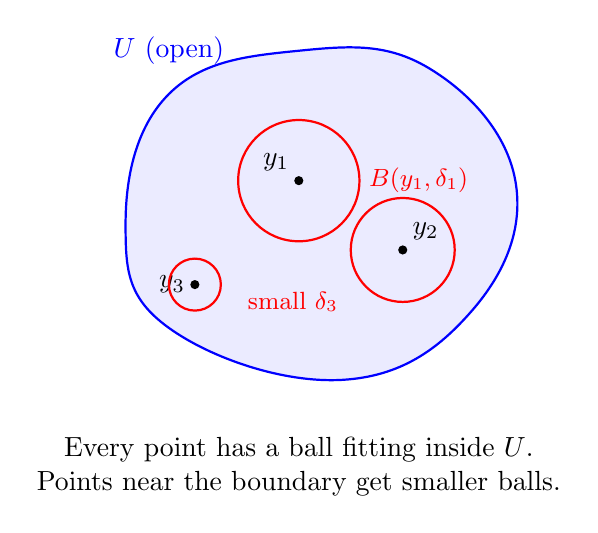
\begin{tikzpicture}[scale=1.1]
    % The open set U (irregular blob)
    \draw[thick, blue, fill=blue!8]
        plot[smooth cycle, tension=0.7] coordinates
        {(-2,0) (-1.5,1.5) (0,2) (1.5,1.8) (2.5,0.5) (2,-1) (0.5,-1.8) (-1.5,-1.2)};
    \node[blue] at (-1.5,2) {$U$ (open)};

    % Point y1 with ball
    \fill (0,0.5) circle (1.5pt) node[above left] {$y_1$};
    \draw[thick, red] (0,0.5) circle (0.7);
    \node[red, right] at (0.7,0.5) {\small $B(y_1, \delta_1)$};

    % Point y2 with ball
    \fill (1.2,-0.3) circle (1.5pt) node[above right] {$y_2$};
    \draw[thick, red] (1.2,-0.3) circle (0.6);

    % Point y3 near boundary with small ball
    \fill (-1.2,-0.7) circle (1.5pt) node[left] {$y_3$};
    \draw[thick, red] (-1.2,-0.7) circle (0.3);
    \node[red, right] at (-0.7,-0.9) {\small small $\delta_3$};

    % Annotation
    \node[align=center] at (0,-2.8) {Every point has a ball fitting inside $U$.\\
    Points near the boundary get smaller balls.};
\end{tikzpicture}
\end{center}

\begin{notebox}
\textbf{Proof strategy (Lecture 4).}
\begin{itemize}
    \item $(\Rightarrow)$ Follows directly from the definition of the topology generated by a basis (open balls are the basis elements).
    \item $(\Leftarrow)$ For each $y \in U$, pick $\delta_y > 0$ with $B(y, \delta_y) \subseteq U$. Then $U = \bigcup_{y \in U} B(y, \delta_y)$. Each ball is a basis element (hence open), and an arbitrary union of open sets is open.
\end{itemize}

This characterization is the bridge between the abstract topology axioms and concrete $\eps$-$\delta$ arguments.
\end{notebox}

\newpage
%======================================================================
% QUESTION 3
%======================================================================
\subsection{Question 3: Interior and Closure of a Set}

\begin{summarybox}
\textbf{Question:} Define the interior and closure of a set.
\end{summarybox}

\subsubsection*{Closure (Lecture 4)}

\textbf{Definition.} The \defn{closure} of a set $E \subseteq X$ is the smallest closed set containing $E$:
\[
\overline{E} = \bigcap \{C \subseteq X : C \text{ is closed and } E \subseteq C\}.
\]

\textbf{Equivalent characterization (Lecture 4):} $x \in \overline{E}$ if and only if every neighborhood of $x$ intersects $E$. That is,
\[
x \in \overline{E} \iff \text{for all open } U \ni x, \quad U \cap E \neq \emptyset.
\]

\textbf{Decomposition (Lecture 4):} $\overline{E} = E \cup E'$, where $E'$ is the set of \defn{limit points} of $E$ (points $x$ such that every neighborhood of $x$ contains a point of $E$ different from $x$).

So the closure takes $E$ and ``adds in'' all the points that $E$ accumulates toward.

\subsubsection*{Interior}

\textbf{Definition.} The \defn{interior} of a set $E \subseteq X$ is the largest open set contained in $E$:
\[
E^\circ = \bigcup \{U \subseteq X : U \text{ is open and } U \subseteq E\}.
\]

\textbf{Equivalent characterization:} $x \in E^\circ$ if and only if there exists an open neighborhood $U$ of $x$ with $U \subseteq E$. In a metric space:
\[
x \in E^\circ \iff \text{there exists } \delta > 0 \text{ such that } B(x, \delta) \subseteq E.
\]

So the interior strips away the ``boundary'' --- the points that are in $E$ but have no room around them.

\subsubsection*{Visual Comparison}

\begin{center}
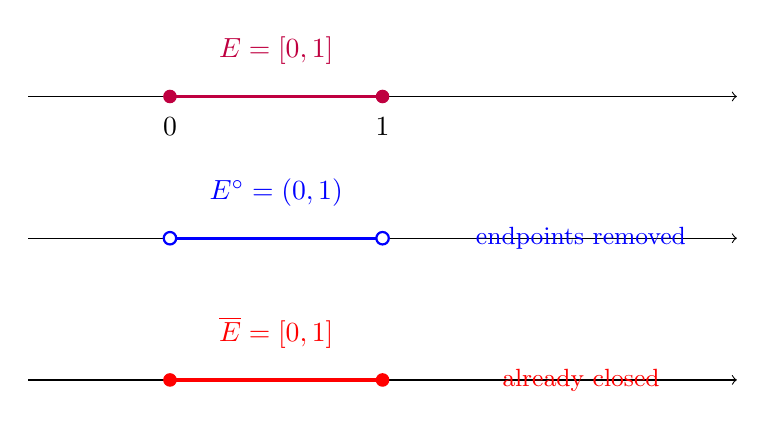
\begin{tikzpicture}[scale=0.9]
    % Original set E = [0, 1]
    \draw[->] (-1,0) -- (9,0) node[right] {$\R$};

    % E = [0, 1] on the number line
    \draw[very thick, purple] (1,0) -- (4,0);
    \filldraw[purple] (1,0) circle (2.5pt);
    \filldraw[purple] (4,0) circle (2.5pt);
    \node[purple, above=8pt] at (2.5,0) {$E = [0, 1]$};
    \node[below=4pt] at (1,0) {$0$};
    \node[below=4pt] at (4,0) {$1$};

    % Interior
    \begin{scope}[yshift=-2.0cm]
        \draw[->] (-1,0) -- (9,0);
        \draw[very thick, blue] (1,0) -- (4,0);
        \filldraw[white, draw=blue, thick] (1,0) circle (2.5pt);
        \filldraw[white, draw=blue, thick] (4,0) circle (2.5pt);
        \node[blue, above=8pt] at (2.5,0) {$E^\circ = (0, 1)$};
        \node[blue] at (6.8,0) {\small endpoints removed};
    \end{scope}

    % Closure
    \begin{scope}[yshift=-4.0cm]
        \draw[->] (-1,0) -- (9,0);
        \draw[very thick, red] (1,0) -- (4,0);
        \filldraw[red] (1,0) circle (2.5pt);
        \filldraw[red] (4,0) circle (2.5pt);
        \node[red, above=8pt] at (2.5,0) {$\overline{E} = [0, 1]$};
        \node[red] at (6.8,0) {\small already closed};
    \end{scope}
\end{tikzpicture}
\end{center}

\medskip

\begin{center}
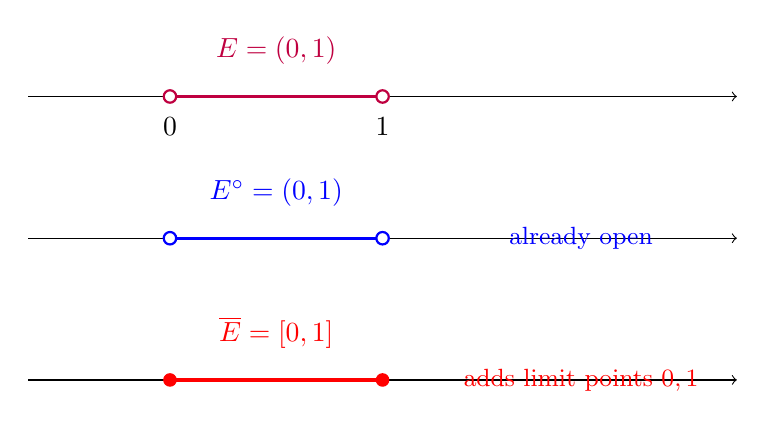
\begin{tikzpicture}[scale=0.9]
    % Original set E = (0, 1)
    \draw[->] (-1,0) -- (9,0) node[right] {$\R$};

    \draw[very thick, purple] (1,0) -- (4,0);
    \filldraw[white, draw=purple, thick] (1,0) circle (2.5pt);
    \filldraw[white, draw=purple, thick] (4,0) circle (2.5pt);
    \node[purple, above=8pt] at (2.5,0) {$E = (0, 1)$};
    \node[below=4pt] at (1,0) {$0$};
    \node[below=4pt] at (4,0) {$1$};

    % Interior
    \begin{scope}[yshift=-2.0cm]
        \draw[->] (-1,0) -- (9,0);
        \draw[very thick, blue] (1,0) -- (4,0);
        \filldraw[white, draw=blue, thick] (1,0) circle (2.5pt);
        \filldraw[white, draw=blue, thick] (4,0) circle (2.5pt);
        \node[blue, above=8pt] at (2.5,0) {$E^\circ = (0, 1)$};
        \node[blue] at (6.8,0) {\small already open};
    \end{scope}

    % Closure
    \begin{scope}[yshift=-4.0cm]
        \draw[->] (-1,0) -- (9,0);
        \draw[very thick, red] (1,0) -- (4,0);
        \filldraw[red] (1,0) circle (2.5pt);
        \filldraw[red] (4,0) circle (2.5pt);
        \node[red, above=8pt] at (2.5,0) {$\overline{E} = [0, 1]$};
        \node[red] at (6.8,0) {\small adds limit points $0, 1$};
    \end{scope}
\end{tikzpicture}
\end{center}

\begin{notebox}
\textbf{Interior and closure are dual.} Just as open and closed sets are complements, interior and closure are related by:
\[
(X \setminus E)^\circ = X \setminus \overline{E}, \qquad \overline{X \setminus E} = X \setminus E^\circ.
\]
The interior ``shrinks'' $E$ to its open core; the closure ``grows'' $E$ to include its boundary. Key relationships:
\begin{center}
\renewcommand{\arraystretch}{1.3}
\begin{tabular}{|c|c|c|}
\hline
\textbf{Property} & \textbf{Interior $E^\circ$} & \textbf{Closure $\overline{E}$} \\
\hline
Definition & Largest open set $\subseteq E$ & Smallest closed set $\supseteq E$ \\
Characterization & $\exists\; B(x,\delta) \subseteq E$ & every nbhd of $x$ meets $E$ \\
Always satisfies & $E^\circ \subseteq E$ & $E \subseteq \overline{E}$ \\
$E$ is open $\iff$ & $E^\circ = E$ & --- \\
$E$ is closed $\iff$ & --- & $\overline{E} = E$ \\
\hline
\end{tabular}
\end{center}
\end{notebox}

\newpage
%======================================================================
% QUESTION 4
%======================================================================
\subsection{Question 4: Connectedness}

\begin{summarybox}
\textbf{Question:} Define connectedness.
\end{summarybox}

\subsubsection*{Separated Sets (Lecture 6)}

\textbf{Definition.} Two subsets $A, B \subset X$ are \defn{separated} if
\[
\overline{A} \cap B = \emptyset \qquad \text{and} \qquad A \cap \overline{B} = \emptyset.
\]

This is stronger than just $A \cap B = \emptyset$ (disjoint). Separated means neither set contains nor ``touches'' limit points of the other. The sets must be truly ``apart'' --- no point of one set is a limit point of the other.

\begin{center}
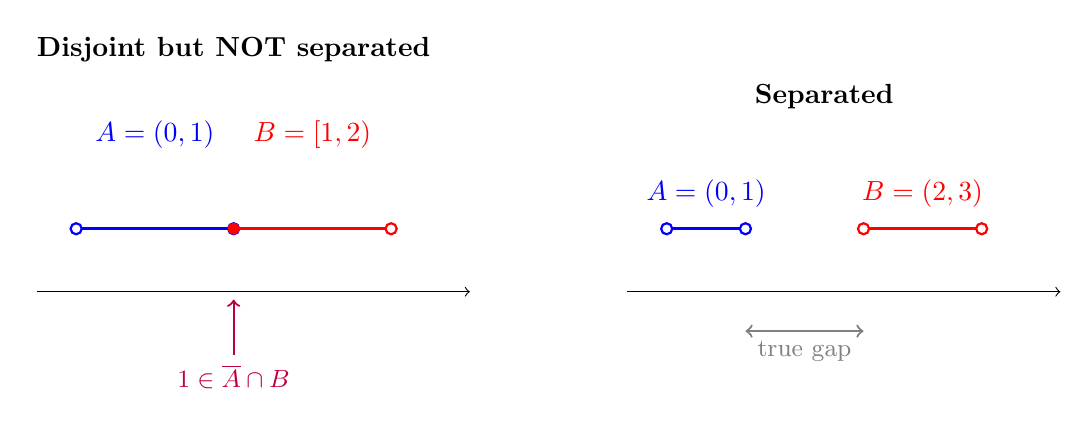
\begin{tikzpicture}[scale=1.0]
    % Disjoint but NOT separated
    \begin{scope}[xshift=0cm]
        \node[above, font=\bfseries] at (2.5, 2.8) {Disjoint but NOT separated};
        \draw[->] (0,0) -- (5.5,0);

        % A = (0,1)
        \draw[very thick, blue] (0.5,0.8) -- (2.5,0.8);
        \filldraw[white, draw=blue, thick] (0.5,0.8) circle (2pt);
        \filldraw[white, draw=blue, thick] (2.5,0.8) circle (2pt);
        \node[blue] at (1.5, 2.0) {$A = (0,1)$};

        % B = [1,2)
        \draw[very thick, red] (2.5,0.8) -- (4.5,0.8);
        \filldraw[red] (2.5,0.8) circle (2pt);
        \filldraw[white, draw=red, thick] (4.5,0.8) circle (2pt);
        \node[red] at (3.5, 2.0) {$B = [1,2)$};

        % Problem point
        \draw[->, thick, purple] (2.5,-0.8) -- (2.5,-0.1);
        \node[purple, below] at (2.5,-0.8) {\small $1 \in \overline{A} \cap B$};
    \end{scope}

    % Separated
    \begin{scope}[xshift=7.5cm]
        \node[above, font=\bfseries] at (2.5, 2.2) {Separated};
        \draw[->] (0,0) -- (5.5,0);

        % A = (0,1)
        \draw[very thick, blue] (0.5,0.8) -- (1.5,0.8);
        \filldraw[white, draw=blue, thick] (0.5,0.8) circle (2pt);
        \filldraw[white, draw=blue, thick] (1.5,0.8) circle (2pt);
        \node[blue, above=4pt] at (1, 0.8) {$A = (0,1)$};

        % B = (2,3)
        \draw[very thick, red] (3,0.8) -- (4.5,0.8);
        \filldraw[white, draw=red, thick] (3,0.8) circle (2pt);
        \filldraw[white, draw=red, thick] (4.5,0.8) circle (2pt);
        \node[red, above=4pt] at (3.75, 0.8) {$B = (2,3)$};

        % Gap
        \draw[<->, thick, gray] (1.5,-0.5) -- (3,-0.5);
        \node[gray, below] at (2.25,-0.5) {\small true gap};
    \end{scope}
\end{tikzpicture}
\end{center}

\subsubsection*{Connected Sets (Lecture 6)}

\textbf{Definition.} A set $E \subset X$ is \defn{connected} if it is \emph{not} the union of two nonempty separated sets. That is, there do \emph{not} exist nonempty $A, B$ with $A \cup B = E$, $\overline{A} \cap B = \emptyset$, and $A \cap \overline{B} = \emptyset$.

Intuitively: $E$ is connected if you cannot split it into two pieces that are truly apart from each other. It is ``all one piece.''

\subsubsection*{Characterization in $\R$ (Lecture 6)}

\textbf{Theorem.} $E \subset \R$ is connected if and only if: for all $x, y \in E$ with $x < z < y$, we have $z \in E$.

In other words, connected subsets of $\R$ are exactly the \textbf{intervals} (possibly unbounded, possibly open/closed/half-open). A connected subset of $\R$ has no ``gaps.''

\begin{center}
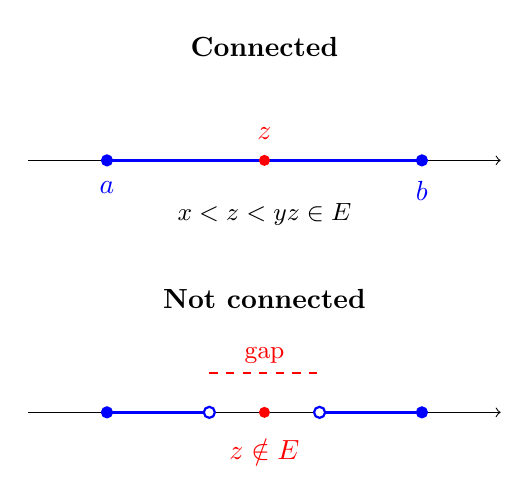
\begin{tikzpicture}[scale=1.0]
    % Connected
    \begin{scope}
        \node[above, font=\bfseries] at (3, 1.2) {Connected};
        \draw[->] (0,0) -- (6,0);
        \draw[very thick, blue] (1,0) -- (5,0);
        \filldraw[blue] (1,0) circle (2pt) node[below=4pt] {$a$};
        \filldraw[blue] (5,0) circle (2pt) node[below=4pt] {$b$};

        % z in between
        \fill[red] (3,0) circle (2pt) node[above=4pt, red] {$z$};
        \node[below=12pt] at (3,0) {\small $x < z < y \implies z \in E$ \checkmark};
    \end{scope}

    % Not connected
    \begin{scope}[yshift=-3.2cm]
        \node[above, font=\bfseries] at (3, 1.2) {Not connected};
        \draw[->] (0,0) -- (6,0);
        \draw[very thick, blue] (1,0) -- (2.3,0);
        \draw[very thick, blue] (3.7,0) -- (5,0);
        \filldraw[blue] (1,0) circle (2pt);
        \filldraw[blue] (5,0) circle (2pt);
        \filldraw[white, draw=blue, thick] (2.3,0) circle (2pt);
        \filldraw[white, draw=blue, thick] (3.7,0) circle (2pt);

        % Gap
        \draw[thick, red, dashed] (2.3,0.5) -- (3.7,0.5);
        \node[red, above] at (3,0.5) {\small gap};
        \fill[red] (3,0) circle (2pt) node[below=6pt, red] {$z \notin E$};
    \end{scope}
\end{tikzpicture}
\end{center}

\begin{notebox}
\textbf{Proof approach (Lecture 6).}

$(\Rightarrow)$ \textbf{Connected $\implies$ no gaps:} Contrapositive. If there is a gap ($x, y \in E$ but $z \notin E$ with $x < z < y$), split $E$ into $A = E \cap (-\infty, z)$ and $B = E \cap (z, \infty)$. Since $z \notin E$, we get $A \cup B = E$. Both are nonempty ($x \in A$, $y \in B$). Since $\overline{A} \subseteq (-\infty, z]$ and $B \subseteq (z, \infty)$, the sets are separated. So $E$ is disconnected.

$(\Leftarrow)$ \textbf{No gaps $\implies$ connected:} Contrapositive. If $E = A \cup B$ with $A, B$ nonempty and separated, pick $x \in A$, $y \in B$ with $x < y$. Let $z = \sup(A \cap [x,y])$. This $z$ (or a point near it) turns out to be in $E$ but creates a contradiction with the separation condition, producing a gap.

The key technique in $(\Leftarrow)$: use the \textbf{supremum} to find the ``boundary'' between $A$ and $B$, then show this boundary point cannot belong to either set.
\end{notebox}

\newpage
%======================================================================
% QUESTION 5
%======================================================================
\subsection{Question 5: Convergence}

\begin{summarybox}
\textbf{Question:} Define convergence.
\end{summarybox}

\subsubsection*{Convergence of a Sequence (Lecture 4)}

\textbf{Definition.} A sequence $(x_n)$ in a topological space $X$ \defn{converges} to $y \in X$ if for every neighborhood $U$ of $y$, there exists $N \in \N$ such that for all $n \geq N$, $x_n \in U$.

In a metric space $(X, d)$, this becomes the familiar $\eps$-$N$ definition:

$(x_n) \to y$ if and only if for every $\eps > 0$, there exists $N \in \N$ such that
\[
n \geq N \implies d(x_n, y) < \eps.
\]

\textbf{Intuition:} No matter how small a ball $B(y, \eps)$ you draw around $y$, eventually (past some index $N$) \emph{all} terms of the sequence land inside that ball. Finitely many terms may be outside, but from some point on, they all stay close.

\begin{center}
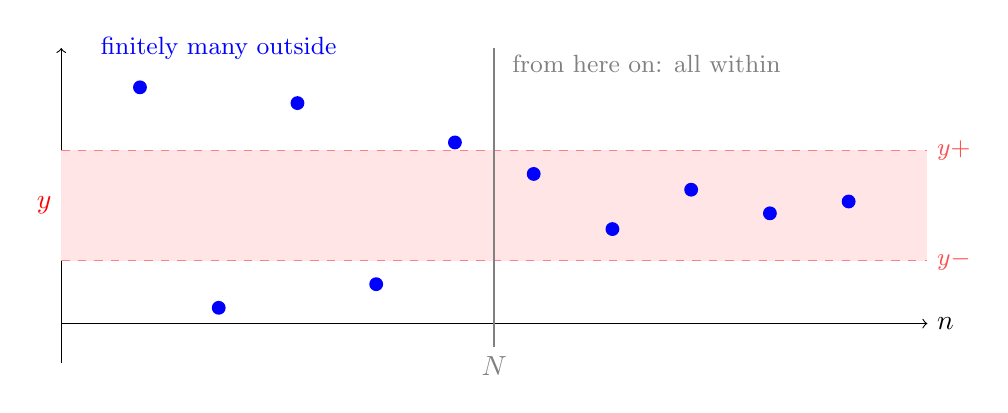
\begin{tikzpicture}[scale=1.0]
    % Axes
    \draw[->] (0,0) -- (11,0) node[right] {$n$};
    \draw[->] (0,-0.5) -- (0,3.5) node[above] {};

    % The limit y
    \draw[dashed, red, thick] (0,1.5) -- (11,1.5);
    \node[red, left] at (0,1.5) {$y$};

    % Epsilon band
    \fill[red!10] (0,0.8) rectangle (11,2.2);
    \draw[dashed, red!50] (0,0.8) -- (11,0.8);
    \draw[dashed, red!50] (0,2.2) -- (11,2.2);
    \node[red!70, right] at (11,2.2) {\small $y + \eps$};
    \node[red!70, right] at (11,0.8) {\small $y - \eps$};

    % Sequence terms (converging)
    \fill[blue] (1, 3.0) circle (2.5pt);
    \fill[blue] (2, 0.2) circle (2.5pt);
    \fill[blue] (3, 2.8) circle (2.5pt);
    \fill[blue] (4, 0.5) circle (2.5pt);
    \fill[blue] (5, 2.3) circle (2.5pt);
    % After N, all inside the band
    \fill[blue] (6, 1.9) circle (2.5pt);
    \fill[blue] (7, 1.2) circle (2.5pt);
    \fill[blue] (8, 1.7) circle (2.5pt);
    \fill[blue] (9, 1.4) circle (2.5pt);
    \fill[blue] (10, 1.55) circle (2.5pt);

    % N marker
    \draw[thick, gray] (5.5,-0.3) -- (5.5,3.5);
    \node[gray, below] at (5.5,-0.3) {$N$};
    \node[gray, right=3pt] at (5.5,3.3) {\small from here on: all within $\eps$};

    % Labels
    \node[blue] at (2,3.5) {\small finitely many outside};
\end{tikzpicture}
\end{center}

\subsubsection*{Key Points}

\begin{itemize}
    \item \textbf{Limit points vs.\ limits of sequences (Lecture 4):} If $p$ is a limit point of $E$, then every neighborhood of $p$ contains \emph{infinitely many} points of $E$ (proved in Lecture 4). This means we can construct a sequence in $E$ converging to $p$.

    \item \textbf{$N$ depends on $\eps$:} Smaller $\eps$ (tighter tolerance) generally requires a larger $N$ (more terms before the sequence settles in). The definition requires that \emph{for every} $\eps$, \emph{some} $N$ exists.

    \item \textbf{Convergence in $\R^n$:} A sequence $(\vec{x}_n)$ in $\R^n$ converges to $\vec{y}$ if and only if each coordinate converges: $\vec{x}_n \to \vec{y}$ iff $x_n^{(i)} \to y^{(i)}$ for all $i = 1, \ldots, n$. (This follows from the equivalence of the product topology and the metric topology on $\R^n$, proved in Lecture 4.)
\end{itemize}

\begin{notebox}
\textbf{Common proof pattern.} To show $(x_n) \to y$:
\begin{enumerate}
    \item \textbf{Let $\eps > 0$ be given.} (You are proving a ``for all $\eps$'' statement.)
    \item \textbf{Find $N$} (usually in terms of $\eps$) such that $d(x_n, y) < \eps$ for $n \geq N$. Often this involves solving an inequality like $\frac{1}{n} < \eps$, giving $N > \frac{1}{\eps}$.
    \item \textbf{Verify:} For $n \geq N$, compute or bound $d(x_n, y)$ and show it is $< \eps$.
\end{enumerate}

The Archimedean property (Lecture 2) guarantees that $N$ exists: for any $\eps > 0$, there is $N \in \N$ with $N > 1/\eps$.
\end{notebox}

\newpage
%======================================================================
% QUESTION 6
%======================================================================
\subsection{Question 6: The Cauchy Criterion}

\begin{summarybox}
\textbf{Question:} State the Cauchy criterion and explain what it means.
\end{summarybox}

\subsubsection*{Statement (Lecture 9)}

\textbf{Definition.} A sequence $\{s_n\}$ in a metric space $(X, d)$ is a \defn{Cauchy sequence} if for every $\eps > 0$, there exists $N \in \N$ such that for all $m, n \geq N$,
\[
d(s_m, s_n) < \eps.
\]

\textbf{Cauchy Criterion.} In $\R$ (or $\R^n$), a sequence converges if and only if it is Cauchy.

\subsubsection*{What It Means}

The standard definition of convergence ($s_n \to s$) requires you to \emph{know the limit $s$} in advance. The Cauchy criterion removes this requirement: instead of checking that terms get close to some target, you check that \emph{terms get close to each other}.

\begin{center}
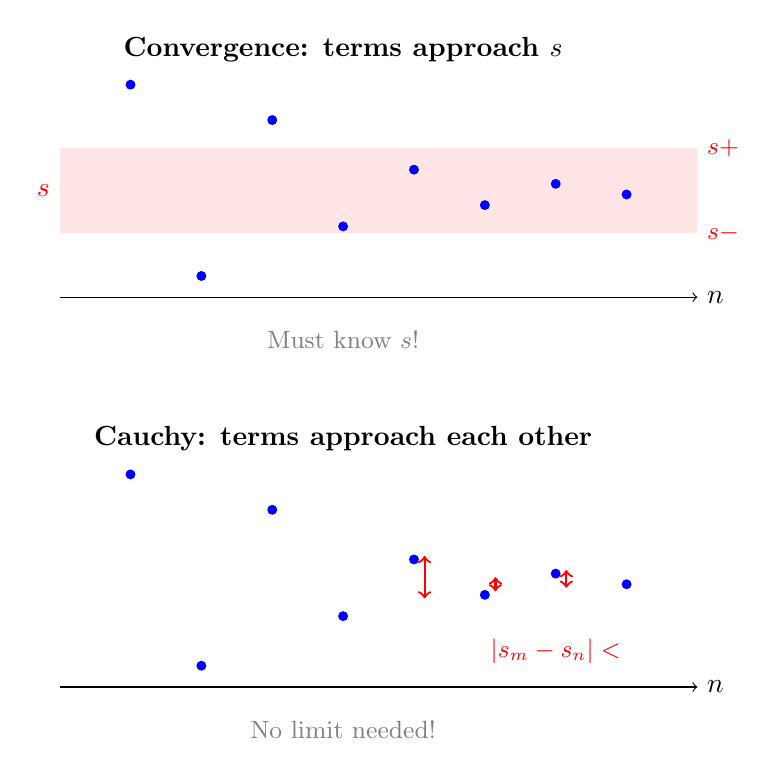
\begin{tikzpicture}[scale=0.9]
    % Top: convergence (need to know limit)
    \begin{scope}
        \node[font=\bfseries] at (4, 3.5) {Convergence: terms approach $s$};
        \draw[->] (0,0) -- (9,0) node[right] {$n$};
        \draw[dashed, red, thick] (0,1.5) -- (9,1.5);
        \node[red, left] at (0,1.5) {$s$};
        \fill[red!10] (0,0.9) rectangle (9,2.1);

        \fill[blue] (1, 3.0) circle (2pt);
        \fill[blue] (2, 0.3) circle (2pt);
        \fill[blue] (3, 2.5) circle (2pt);
        \fill[blue] (4, 1.0) circle (2pt);
        \fill[blue] (5, 1.8) circle (2pt);
        \fill[blue] (6, 1.3) circle (2pt);
        \fill[blue] (7, 1.6) circle (2pt);
        \fill[blue] (8, 1.45) circle (2pt);

        \node[red, right] at (9, 2.1) {\small $s + \eps$};
        \node[red, right] at (9, 0.9) {\small $s - \eps$};
        \node[gray] at (4, -0.6) {\small Must know $s$!};
    \end{scope}

    % Bottom: Cauchy (don't need limit)
    \begin{scope}[yshift=-5.5cm]
        \node[font=\bfseries] at (4, 3.5) {Cauchy: terms approach each other};
        \draw[->] (0,0) -- (9,0) node[right] {$n$};

        \fill[blue] (1, 3.0) circle (2pt);
        \fill[blue] (2, 0.3) circle (2pt);
        \fill[blue] (3, 2.5) circle (2pt);
        \fill[blue] (4, 1.0) circle (2pt);
        \fill[blue] (5, 1.8) circle (2pt);
        \fill[blue] (6, 1.3) circle (2pt);
        \fill[blue] (7, 1.6) circle (2pt);
        \fill[blue] (8, 1.45) circle (2pt);

        % Bracket showing close terms
        \draw[<->, thick, red] (5.15, 1.85) -- (5.15, 1.25);
        \draw[<->, thick, red] (6.15, 1.35) -- (6.15, 1.55);
        \draw[<->, thick, red] (7.15, 1.65) -- (7.15, 1.4);

        \node[red] at (7, 0.5) {\small $|s_m - s_n| < \eps$};
        \node[gray] at (4, -0.6) {\small No limit needed!};
    \end{scope}
\end{tikzpicture}
\end{center}

\subsubsection*{Why This Matters}

\begin{enumerate}
    \item \textbf{Practical:} For many sequences (especially series), computing the exact limit is hard or impossible. The Cauchy criterion lets you prove convergence anyway.

    \item \textbf{For series (Lecture 9):} If $s_n = \sum_{k=0}^n a_k$ are partial sums, the Cauchy condition becomes: for every $\eps > 0$, there exists $N$ such that for all $m > n \geq N$,
    \[
    \left|\sum_{k=n+1}^{m} a_k\right| < \eps.
    \]
    This says: the ``tail sums'' become arbitrarily small.

    \item \textbf{Completeness:} The fact that Cauchy $\iff$ convergent is a property of $\R$, not of all metric spaces. A metric space where every Cauchy sequence converges is called \defn{complete}. The rationals $\Q$ are \emph{not} complete: the sequence $1, 1.4, 1.41, 1.414, \ldots$ is Cauchy in $\Q$ but converges to $\sqrt{2} \notin \Q$. This connects back to Question 1: $\R$ is the \emph{completion} of $\Q$.
\end{enumerate}

\begin{notebox}
\textbf{Key corollary:} If $\sum a_n$ converges, taking $m = n+1$ in the Cauchy condition gives $|a_{n+1}| < \eps$ for large $n$, so $a_n \to 0$. The converse is false: $\sum 1/n$ diverges even though $1/n \to 0$ (the harmonic series).
\end{notebox}

\newpage
%======================================================================
% QUESTION 7
%======================================================================
\subsection{Question 7: Sequential Compactness}

\begin{summarybox}
\textbf{Question:} Define sequential compactness and its broader meaning.
\end{summarybox}

\subsubsection*{Definition}

A set $K$ is \defn{sequentially compact} if every sequence in $K$ has a subsequence that converges to a point in $K$.

\subsubsection*{Relation to Compactness (Lecture 5)}

In $\R^n$, the Heine--Borel theorem gives three equivalent characterizations:

\begin{center}
\renewcommand{\arraystretch}{1.5}
\begin{tabular}{|c|p{9cm}|}
\hline
\textbf{(1)} & $K$ is \textbf{closed and bounded} \\
\hline
\textbf{(2)} & $K$ is \textbf{compact}: every open cover has a finite subcover \\
\hline
\textbf{(3)} & Every \textbf{infinite subset} of $K$ has a limit point in $K$ \\
\hline
\end{tabular}
\end{center}

Condition (3) is essentially sequential compactness. If every infinite subset has a limit point in $K$, then given any sequence $(x_n)$ in $K$:
\begin{itemize}
    \item If the sequence takes infinitely many distinct values, that infinite subset has a limit point $p \in K$, and we can extract a subsequence converging to $p$.
    \item If the sequence takes only finitely many values, some value repeats infinitely often, giving a constant (hence convergent) subsequence.
\end{itemize}

\begin{center}
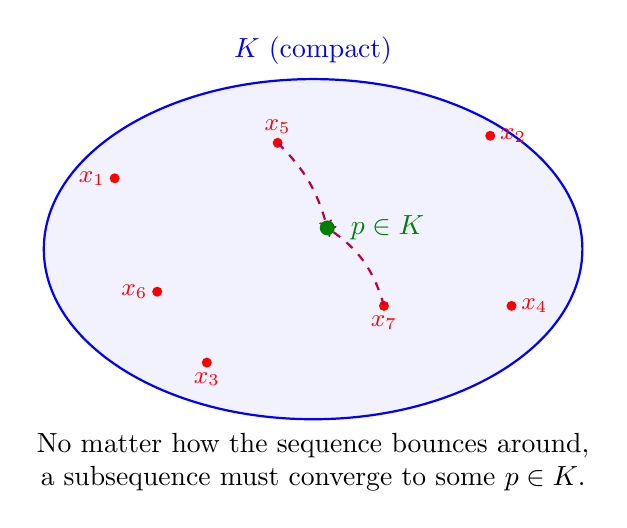
\begin{tikzpicture}[scale=0.9]
    % Compact set
    \draw[thick, blue, fill=blue!5] (0,0) ellipse (3.8 and 2.4);
    \node[blue] at (0, 2.8) {$K$ (compact)};

    % Sequence terms bouncing around (spread out to edges)
    \fill[red] (-2.8, 1.0) circle (2pt) node[left] {\small $x_1$};
    \fill[red] (2.5, 1.6) circle (2pt) node[right] {\small $x_2$};
    \fill[red] (-1.5, -1.6) circle (2pt) node[below] {\small $x_3$};
    \fill[red] (2.8, -0.8) circle (2pt) node[right] {\small $x_4$};
    \fill[red] (-0.5, 1.5) circle (2pt) node[above] {\small $x_5$};
    \fill[red] (-2.2, -0.6) circle (2pt) node[left] {\small $x_6$};
    \fill[red] (1.0, -0.8) circle (2pt) node[below] {\small $x_7$};

    % Subsequence converging (arrows from x5 and x7 toward p)
    \draw[->, thick, purple, dashed] (-0.5, 1.5) to[bend left=15] (0.2, 0.3);
    \draw[->, thick, purple, dashed] (1.0, -0.8) to[bend right=20] (0.2, 0.3);

    % Limit point (centered, with space around it)
    \fill[green!50!black] (0.2, 0.3) circle (3pt);
    \node[green!50!black, right=5pt] at (0.2, 0.3) {$p \in K$};

    \node[align=center] at (0, -3) {No matter how the sequence bounces around,\\
    a subsequence must converge to some $p \in K$.};
\end{tikzpicture}
\end{center}

\subsubsection*{Broader Meaning}

Sequential compactness means a compact set is ``inescapable'': any infinite process (sequence) that stays in $K$ must eventually cluster somewhere in $K$. You cannot have a sequence that keeps running away or spreading out.

This is why compactness is so powerful:
\begin{itemize}
    \item \textbf{Extreme Value Theorem:} Continuous functions on compact sets attain max/min (the optimizing sequence must have a convergent subsequence).
    \item \textbf{Uniform continuity:} Continuous functions on compact sets are uniformly continuous (used in Lecture 6).
    \item \textbf{Bolzano--Weierstrass:} Every bounded sequence in $\R^n$ has a convergent subsequence (the Weierstrass theorem from Lecture 5).
\end{itemize}

\newpage
%======================================================================
% QUESTION 8
%======================================================================
\subsection{Question 8: Convergence of a Sequence and a Series}

\begin{summarybox}
\textbf{Question:} Define convergence of a sequence and of a series.
\end{summarybox}

\subsubsection*{Convergence of a Sequence (Lecture 4)}

\textbf{Definition.} A sequence $(x_n)$ in a metric space $(X, d)$ \defn{converges} to $y \in X$, written $x_n \to y$, if for every $\eps > 0$ there exists $N \in \N$ such that
\[
n \geq N \implies d(x_n, y) < \eps.
\]

\subsubsection*{Convergence of a Series (Lecture 9)}

A series is \emph{not} a new object --- it is a sequence of partial sums.

\textbf{Definition.} Given a sequence $\{a_n\}$, the \defn{partial sums} are
\[
s_n = \sum_{k=0}^{n} a_k = a_0 + a_1 + \cdots + a_n.
\]
The series $\sum_{n=0}^{\infty} a_n$ \defn{converges} to $s$ if the sequence of partial sums converges: $s_n \to s$.

\begin{center}
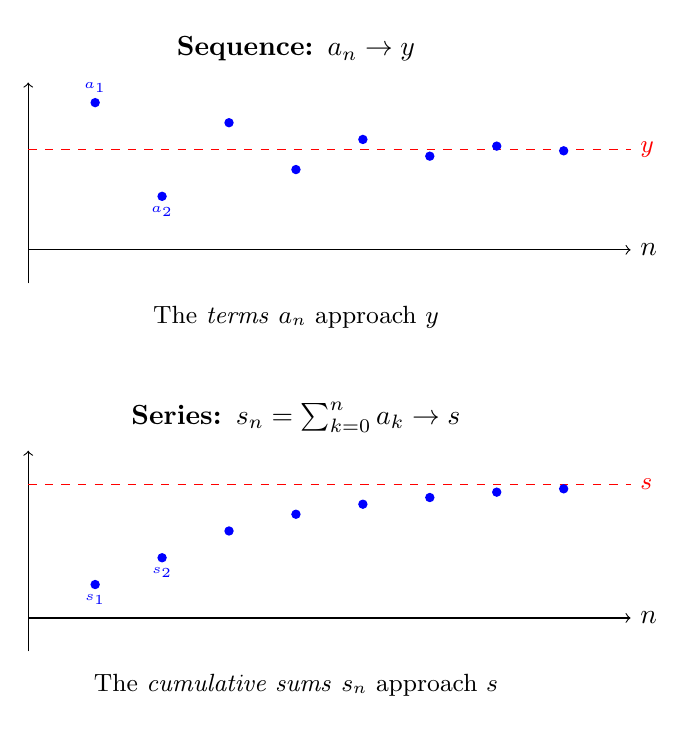
\begin{tikzpicture}[scale=0.85]
    % Sequence (top)
    \begin{scope}
        \node[font=\bfseries] at (4, 3) {Sequence: $a_n \to y$};
        \draw[->] (0,0) -- (9,0) node[right] {$n$};
        \draw[->] (0,-0.5) -- (0,2.5);
        \draw[dashed, red] (0,1.5) -- (9,1.5) node[right] {\small $y$};

        \fill[blue] (1, 2.2) circle (2pt) node[above] {\tiny $a_1$};
        \fill[blue] (2, 0.8) circle (2pt) node[below] {\tiny $a_2$};
        \fill[blue] (3, 1.9) circle (2pt);
        \fill[blue] (4, 1.2) circle (2pt);
        \fill[blue] (5, 1.65) circle (2pt);
        \fill[blue] (6, 1.4) circle (2pt);
        \fill[blue] (7, 1.55) circle (2pt);
        \fill[blue] (8, 1.48) circle (2pt);

        \node at (4, -1) {\small The \emph{terms} $a_n$ approach $y$};
    \end{scope}

    % Series (bottom)
    \begin{scope}[yshift=-5.5cm]
        \node[font=\bfseries] at (4, 3) {Series: $s_n = \sum_{k=0}^n a_k \to s$};
        \draw[->] (0,0) -- (9,0) node[right] {$n$};
        \draw[->] (0,-0.5) -- (0,2.5);
        \draw[dashed, red] (0,2.0) -- (9,2.0) node[right] {\small $s$};

        % Partial sums increasing toward s
        \fill[blue] (1, 0.5) circle (2pt) node[below] {\tiny $s_1$};
        \fill[blue] (2, 0.9) circle (2pt) node[below] {\tiny $s_2$};
        \fill[blue] (3, 1.3) circle (2pt);
        \fill[blue] (4, 1.55) circle (2pt);
        \fill[blue] (5, 1.7) circle (2pt);
        \fill[blue] (6, 1.8) circle (2pt);
        \fill[blue] (7, 1.88) circle (2pt);
        \fill[blue] (8, 1.93) circle (2pt);

        \node at (4, -1) {\small The \emph{cumulative sums} $s_n$ approach $s$};
    \end{scope}
\end{tikzpicture}
\end{center}

\begin{notebox}
\textbf{Key distinction.} ``$a_n \to 0$'' and ``$\sum a_n$ converges'' are \emph{different} statements.
\begin{itemize}
    \item If $\sum a_n$ converges, then $a_n \to 0$ (necessary condition, proved via the Cauchy criterion with $m = n+1$).
    \item The converse is \textbf{false}: $a_n = 1/n \to 0$, but $\sum 1/n = \infty$ (harmonic series diverges).
\end{itemize}
So $a_n \to 0$ is necessary but not sufficient for convergence of the series.
\end{notebox}

\newpage
%======================================================================
% QUESTION 9
%======================================================================
\subsection{Question 9: Convergent Sequences are Bounded}

\begin{summarybox}
\textbf{Question:} Prove that convergent sequences are bounded.
\end{summarybox}

\subsubsection*{Statement}

\textbf{Theorem.} If $(x_n) \to y$ in a metric space $(X, d)$, then the sequence $(x_n)$ is bounded: there exists $M > 0$ such that $d(x_n, y) \leq M$ for all $n$.

\subsubsection*{Concepts Involved}

\begin{itemize}
    \item \textbf{Convergence (Lecture 4):} $x_n \to y$ means for every $\eps > 0$, there exists $N$ such that $d(x_n, y) < \eps$ for all $n \geq N$.
    \item \textbf{Boundedness (Lecture 4):} A set $E$ is bounded if $E \subseteq B(x, M)$ for some $x \in X$ and $M > 0$.
\end{itemize}

\subsubsection*{Proof Approach}

The idea is simple: convergence controls the \emph{tail} (all terms past some $N$), and the \emph{head} (finitely many initial terms) is automatically bounded.

\begin{center}
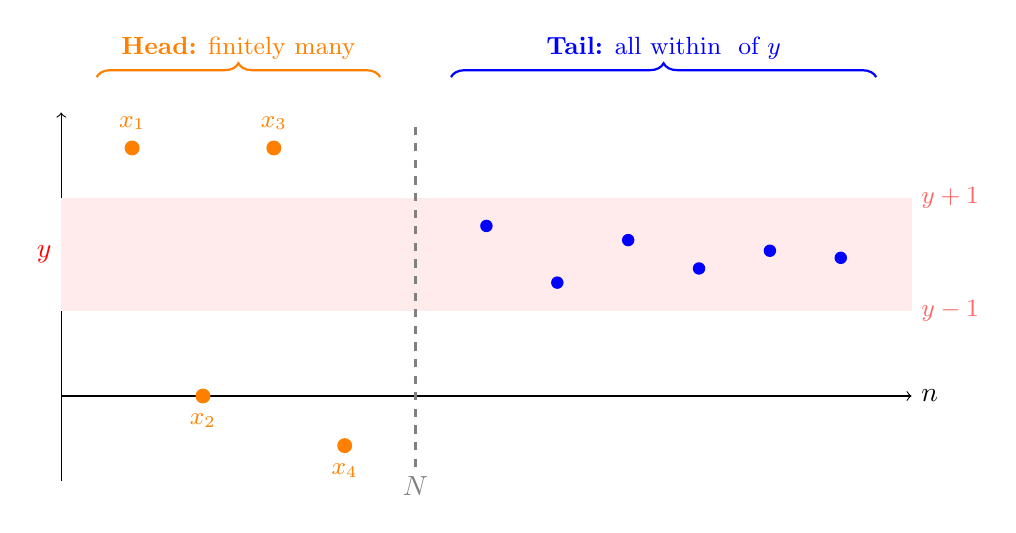
\begin{tikzpicture}[scale=0.9]
    \draw[->] (0,0) -- (12,0) node[right] {$n$};
    \draw[->] (0,-1.2) -- (0,4);

    % The limit
    \draw[dashed, red, thick] (0,2) -- (12,2);
    \node[red, left] at (0,2) {$y$};

    % Epsilon band
    \fill[red!8] (0,1.2) rectangle (12,2.8);
    \node[red!60, right] at (12, 2.8) {\small $y + 1$};
    \node[red!60, right] at (12, 1.2) {\small $y - 1$};

    % Head: finitely many terms (possibly wild)
    \fill[orange] (1, 3.5) circle (3pt) node[above=3pt] {\small $x_1$};
    \fill[orange] (2, 0.0) circle (3pt) node[below=3pt] {\small $x_2$};
    \fill[orange] (3, 3.5) circle (3pt) node[above=3pt] {\small $x_3$};
    \fill[orange] (4, -0.7) circle (3pt) node[below=3pt] {\small $x_4$};

    % N marker
    \draw[thick, gray, dashed] (5,-1.0) -- (5,3.8);
    \node[gray, below] at (5,-1.0) {$N$};

    % Tail: all within eps of y
    \fill[blue] (6, 2.4) circle (2.5pt);
    \fill[blue] (7, 1.6) circle (2.5pt);
    \fill[blue] (8, 2.2) circle (2.5pt);
    \fill[blue] (9, 1.8) circle (2.5pt);
    \fill[blue] (10, 2.05) circle (2.5pt);
    \fill[blue] (11, 1.95) circle (2.5pt);

    % Labels (braces above the points)
    \draw[thick, orange, decorate, decoration={brace, amplitude=5pt}] (0.5,4.5) -- (4.5,4.5);
    \node[orange, above=3pt] at (2.5, 4.5) {\small \textbf{Head:} finitely many};

    \draw[thick, blue, decorate, decoration={brace, amplitude=5pt}] (5.5,4.5) -- (11.5,4.5);
    \node[blue, above=3pt] at (8.5, 4.5) {\small \textbf{Tail:} all within $\eps$ of $y$};
\end{tikzpicture}
\end{center}

\begin{enumerate}
    \item \textbf{Use $\eps = 1$} in the convergence definition: there exists $N$ such that $d(x_n, y) < 1$ for all $n \geq N$.
    \item \textbf{The tail is bounded:} All terms with $n \geq N$ satisfy $d(x_n, y) < 1$.
    \item \textbf{The head is finite:} The terms $x_1, x_2, \ldots, x_{N-1}$ are finitely many, so $\max\{d(x_1, y), \ldots, d(x_{N-1}, y)\}$ is finite.
    \item \textbf{Combine:} Let $M = \max\{d(x_1, y), \ldots, d(x_{N-1}, y), 1\}$. Then $d(x_n, y) \leq M$ for all $n$.
\end{enumerate}

\begin{notebox}
\textbf{Why this works.} The key insight is the split into ``finitely many'' and ``eventually all.'' Convergence gives you control over the tail. The head is automatically tamed because \emph{any finite set is bounded}. Taking the max combines both.

This is a very common pattern in analysis: control the tail by the definition, and handle the (finite) head separately.
\end{notebox}

\newpage
%======================================================================
% QUESTION 10
%======================================================================
\subsection{Question 10: Continuity}

\begin{summarybox}
\textbf{Question:} Define continuity.
\end{summarybox}

\subsubsection*{The Topological Definition (Lecture 6)}

\textbf{Definition.} A function $f : X \to Y$ between topological spaces is \defn{continuous} if for every open set $V \subseteq Y$, the preimage $f^{-1}(V)$ is open in $X$.

This is the most general definition. It says: open sets in the codomain ``pull back'' to open sets in the domain.

\begin{center}
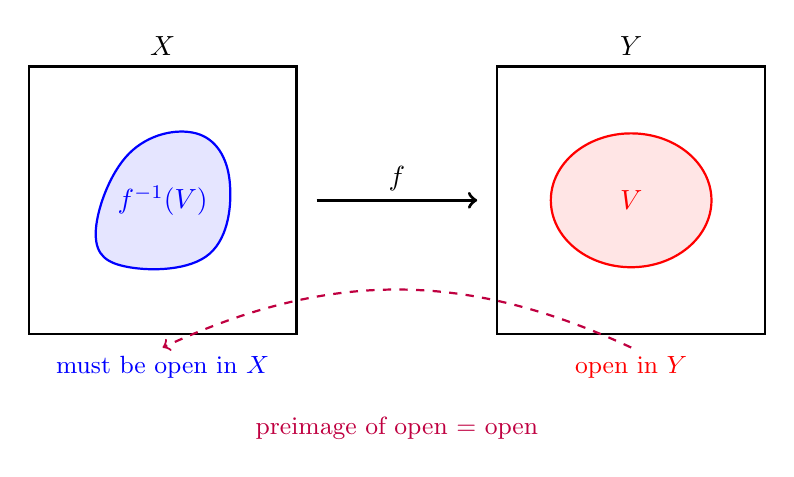
\begin{tikzpicture}[scale=0.85]
    % Domain X
    \draw[thick] (-0.5,-1.5) rectangle (3.5, 2.5);
    \node at (1.5, 2.8) {$X$};

    % Codomain Y
    \draw[thick] (6.5,-1.5) rectangle (10.5, 2.5);
    \node at (8.5, 2.8) {$Y$};

    % Arrow f
    \draw[->, very thick] (3.8, 0.5) -- (6.2, 0.5);
    \node[above] at (5, 0.5) {$f$};

    % V open in Y
    \draw[thick, red, fill=red!10] (8.5, 0.5) ellipse (1.2 and 1.0);
    \node[red] at (8.5, 0.5) {$V$};
    \node[red] at (8.5, -2.0) {\small open in $Y$};

    % f^{-1}(V) open in X
    \draw[thick, blue, fill=blue!10]
        plot[smooth cycle, tension=0.7] coordinates
        {(0.5,0) (1,1.2) (2,1.5) (2.5,0.8) (2.2,-0.3) (1,-0.5)};
    \node[blue] at (1.5, 0.5) {$f^{-1}(V)$};
    \node[blue] at (1.5, -2.0) {\small must be open in $X$};

    % Dashed arrow
    \draw[->, dashed, thick, purple] (8.5, -1.7) to[bend right=25] (1.5, -1.7);
    \node[purple, below] at (5, -2.6) {\small preimage of open = open};
\end{tikzpicture}
\end{center}

\subsubsection*{Three Equivalent Formulations (Lecture 6)}

\begin{enumerate}
    \item \textbf{Basis formulation:} Given a basis $\mathcal{B}$ for the topology on $Y$, $f$ is continuous if and only if $f^{-1}(B)$ is open in $X$ for every $B \in \mathcal{B}$. (You only need to check basis elements, not all open sets.)

    \item \textbf{Local formulation:} $f$ is \defn{continuous at a point $p$} if for every open $V \ni f(p)$ in $Y$, there exists open $U \ni p$ in $X$ with $f(U) \subseteq V$. Then $f$ is continuous (globally) if and only if $f$ is continuous at every point.

    \item \textbf{$\eps$-$\delta$ formulation (metric spaces):} $f$ is continuous at $p$ if for every $\eps > 0$ there exists $\delta > 0$ such that
    \[
    d_X(x, p) < \delta \implies d_Y(f(x), f(p)) < \eps.
    \]
\end{enumerate}

\begin{center}
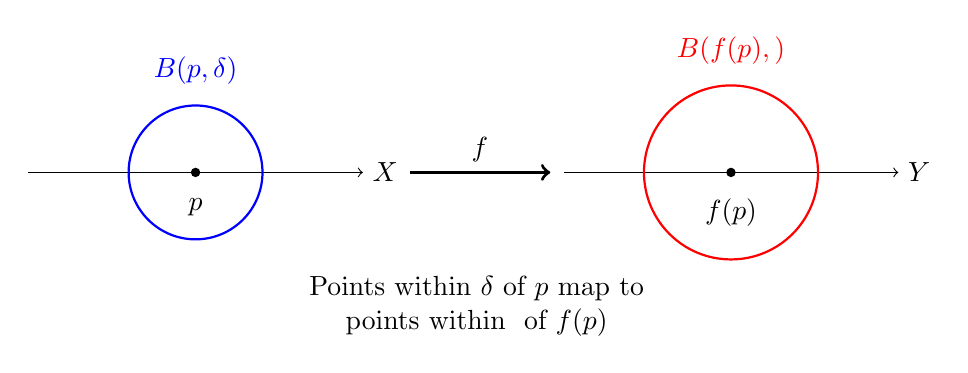
\begin{tikzpicture}[scale=0.85]
    % Domain
    \draw[->] (-0.5,0) -- (4.5,0) node[right] {$X$};
    \fill (2,0) circle (2pt) node[below=6pt] {$p$};

    % Delta ball
    \draw[thick, blue] (2,0) circle (1);
    \node[blue, above=4pt] at (2, 1) {$B(p, \delta)$};

    % Arrow
    \draw[->, very thick] (5.2, 0) -- (7.3, 0) node[midway, above] {$f$};

    % Codomain
    \begin{scope}[xshift=8cm]
        \draw[->] (-0.5,0) -- (4.5,0) node[right] {$Y$};
        \fill (2,0) circle (2pt) node[below=6pt] {$f(p)$};

        % Epsilon ball
        \draw[thick, red] (2,0) circle (1.3);
        \node[red, above=4pt] at (2, 1.3) {$B(f(p), \eps)$};
    \end{scope}

    % Description
    \node[align=center] at (6.2, -2.0) {Points within $\delta$ of $p$ map to\\
    points within $\eps$ of $f(p)$};
\end{tikzpicture}
\end{center}

\begin{notebox}
\textbf{Intuition.} Continuity means ``small changes in input produce small changes in output.'' The $\eps$-$\delta$ definition makes this precise: you choose how close you want outputs to be ($\eps$), and I find how close inputs need to be ($\delta$).

\textbf{The quantifier order matters:}
\[
\underbrace{\forall \eps > 0}_{\text{you pick tolerance}} \quad \underbrace{\exists \delta > 0}_{\text{I find a response}} \quad \underbrace{\forall x: d(x,p) < \delta \implies d(f(x),f(p)) < \eps}_{\text{guarantee}}
\]
Crucially, $\delta$ is allowed to depend on both $\eps$ \emph{and} $p$. This is what distinguishes continuity from \textbf{uniform continuity} (Question~11), where $\delta$ must work for all $p$ simultaneously.
\end{notebox}

\newpage
%======================================================================
% QUESTION 11
%======================================================================
\subsection{Question 11: Continuous Functions on Compact and Connected Sets}

\begin{summarybox}
\textbf{Question:} What is the effect of a continuous function on a compact/connected set?
\end{summarybox}

\subsubsection*{The Main Theorems (Lecture 6)}

\textbf{Theorem.} If $f : X \to Y$ is continuous and $K \subseteq X$ is \textbf{compact}, then $f(K)$ is compact.

\textbf{Theorem.} If $f : X \to Y$ is continuous and $E \subseteq X$ is \textbf{connected}, then $f(E)$ is connected.

In short: \emph{continuous functions preserve compactness and connectedness.}

\subsubsection*{Compactness Is Preserved}

\begin{center}
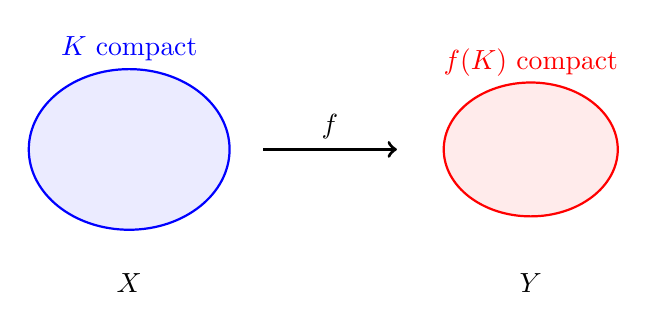
\begin{tikzpicture}[scale=0.85]
    % Domain
    \draw[thick, blue, fill=blue!8] (1.5, 0.5) ellipse (1.5 and 1.2);
    \node[blue] at (1.5, 2) {$K$ compact};
    \node at (1.5, -1.5) {$X$};

    % Arrow
    \draw[->, very thick] (3.5, 0.5) -- (5.5, 0.5) node[midway, above] {$f$};

    % Codomain
    \draw[thick, red, fill=red!8] (7.5, 0.5) ellipse (1.3 and 1.0);
    \node[red] at (7.5, 1.8) {$f(K)$ compact};
    \node at (7.5, -1.5) {$Y$};
\end{tikzpicture}
\end{center}

\textbf{Proof idea (Lecture 6):} Start with an open cover $\{V_\alpha\}$ of $f(K)$. Pull back: $\{f^{-1}(V_\alpha)\}$ is an open cover of $K$ (by continuity). Extract a finite subcover (by compactness of $K$). Push forward: the corresponding $V_{\alpha_i}$'s cover $f(K)$.

\subsubsection*{Consequences of Preserving Compactness}

\textbf{1. Extreme Value Theorem (Lecture 6).} If $f : K \to \R$ is continuous and $K$ is compact, then $f$ attains its maximum and minimum.

\emph{Why:} $f(K)$ is compact in $\R$, hence closed and bounded (Heine--Borel). Bounded means $\sup f(K)$ and $\inf f(K)$ are finite. Closed means $f(K)$ contains its limit points, so $\sup f(K) \in f(K)$ and $\inf f(K) \in f(K)$.

\textbf{2. Uniform Continuity (Lecture 6).} If $f : K \to Y$ is continuous and $K$ is compact, then $f$ is uniformly continuous.

\emph{Recall:} $f$ is uniformly continuous if $\delta$ can be chosen independent of the point $p$:
\[
\forall \eps > 0\;\; \exists \delta > 0 \;\;\text{such that}\;\; d(p,q) < \delta \implies d(f(p), f(q)) < \eps \quad \forall p, q \in K.
\]

\emph{Why compactness helps:} At each point $p$, continuity gives a $\delta_p$. Cover $K$ by balls $B(p, \delta_p/2)$, extract a finite subcover, and take $\delta = \frac{1}{2}\min(\delta_{p_1}, \ldots, \delta_{p_n})$.

\subsubsection*{Connectedness Is Preserved}

\textbf{Proof idea (Lecture 6):} If $f(E)$ were disconnected as $A \cup B$ (separated), then $f^{-1}(A) \cap E$ and $f^{-1}(B) \cap E$ would separate $E$, contradicting the connectedness of $E$.

\subsubsection*{Consequence: Intermediate Value Theorem}

\textbf{IVT (Lecture 6).} If $f : [a,b] \to \R$ is continuous and $f(a) < c < f(b)$, then there exists $p \in (a,b)$ with $f(p) = c$.

\emph{Why:} $[a,b]$ is connected. So $f([a,b])$ is connected in $\R$. Connected subsets of $\R$ are intervals (have no gaps). Since $f(a)$ and $f(b)$ are in $f([a,b])$, every value between them is too.

\begin{center}
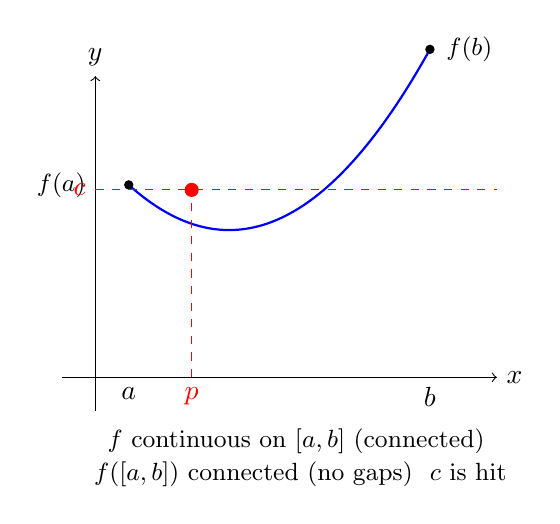
\begin{tikzpicture}[scale=0.85]
    % Axes
    \draw[->] (-0.5, 0) -- (6, 0) node[right] {$x$};
    \draw[->] (0, -0.5) -- (0, 4.5) node[above] {$y$};

    % Function
    \draw[thick, blue, domain=0.5:5, samples=100] plot (\x, {0.3*(\x-1)*(\x-3) + 2.5});

    % Endpoints
    \fill (0.5, {0.3*(0.5-1)*(0.5-3) + 2.5}) circle (2pt);
    \fill (5, {0.3*(5-1)*(5-3) + 2.5}) circle (2pt);
    \node[left] at (0, {0.3*(0.5-1)*(0.5-3) + 2.5}) {\small $f(a)$};
    \node[right] at (5.1, {0.3*(5-1)*(5-3) + 2.5}) {\small $f(b)$};

    % c value
    \draw[dashed, red] (0, 2.8) -- (6, 2.8);
    \node[red, left] at (0, 2.8) {$c$};

    % Intersection point
    \fill[red] (1.44, 2.8) circle (3pt);
    \draw[dashed, red] (1.44, 0) -- (1.44, 2.8);
    \node[red, below] at (1.44, 0) {$p$};

    % Labels
    \node[below] at (0.5, 0) {$a$};
    \node[below] at (5, 0) {$b$};

    \node[align=center] at (3, -1.2) {\small $f$ continuous on $[a,b]$ (connected)\\
    \small $\implies$ $f([a,b])$ connected (no gaps) $\implies$ $c$ is hit};
\end{tikzpicture}
\end{center}

\begin{notebox}
\textbf{Summary table.}
\begin{center}
\renewcommand{\arraystretch}{1.4}
\begin{tabular}{|c|c|c|}
\hline
\textbf{$K$ is\ldots} & \textbf{$f(K)$ is\ldots} & \textbf{Consequence} \\
\hline
Compact & Compact & Extreme Value Thm, Uniform Continuity \\
\hline
Connected & Connected & Intermediate Value Theorem \\
\hline
\end{tabular}
\end{center}

\textbf{What compactness does NOT preserve (Lecture 6):} On a non-compact set $E$, a continuous function can be (1) unbounded, (2) bounded but miss its sup, or (3) not uniformly continuous. All three pathologies are eliminated by compactness.
\end{notebox}

\end{document}
